\chapter{Практические задания}
\section{Задание №1}
В одной программе написать правила, позволяющие найти:
\begin{enumerate}
	\item максимум из двух чисел 
		\begin{itemize}
			\item без использования отсечения;
			\item с использованием отсечения.
		\end{itemize}
	\item максимум из трех чисел
		\begin{itemize}
			\item без использования отсечения;
			\item с использованием отсечения.
		\end{itemize}
\end{enumerate}

Убедиться в правильности результатов.

Для каждого случая пункта 2 обосновать необходимость всех условий тела.
Для одного из вариантов ВОПРОСА и каждого варианта задания 2 составить
таблицу, отражающую конкретный порядок работы системы.

Код программы представлен на листинге \ref{lst:code}.
\newpage
\begin{lstlisting}[label=lst:code, basicstyle=\footnotesize, caption=Код программы]
domains
	number = integer
predicates
	max_from_two(number, number, number)
	max_from_two_cut(number, number, number)
	max_from_three(number, number, number, number)
	max_from_three_cut(number, number, number, number)
clauses
	max_from_two(Number_1, Number_2, Number_1) :- Number_1 >= Number_2.
	max_from_two(Number_1, Number_2, Number_2) :- Number_2 > Number_1.
	
	max_from_two_cut(Number_1, Number_2, Number_1) :- Number_1 >= Number_2, !.
	max_from_two_cut(_, Number_2, Number_2).
	
	max_from_three(Number_1, Number_2, Number_3, Number_1) :- Number_1 >= Number_2, Number_1 >= Number_3.
	max_from_three(Number_1, Number_2, Number_3, Number_2) :- Number_2 >= Number_1, Number_2 >= Number_3.
	max_from_three(Number_1, Number_2, Number_3, Number_3) :- Number_3 >= Number_2, Number_3 >= Number_1.
	
	max_from_three_cut(Number_1, Number_2, Number_3, Number_1) :- Number_1 >= Number_2, Number_1 >= Number_3, !.
	max_from_three_cut(_, Number_2, Number_3, Number_2) :- Number_2 >= Number_3, !.
	max_from_three_cut(_, _, Number_3, Number_3).
goal
	%max_from_two(4, 5, Max_number).
	%max_from_two_cut(4, 5, Max_number).
	%max_from_three(3, 4, 1, Max_number).
	%max_from_three_cut(3, 2, 4, Max_number).
\end{lstlisting}

Ниже на рисунке \ref{image:table_1} приведена таблица порядка поиска ответа для задания 2 (без отсечения):
\begin{figure}[H]
	\centering{
		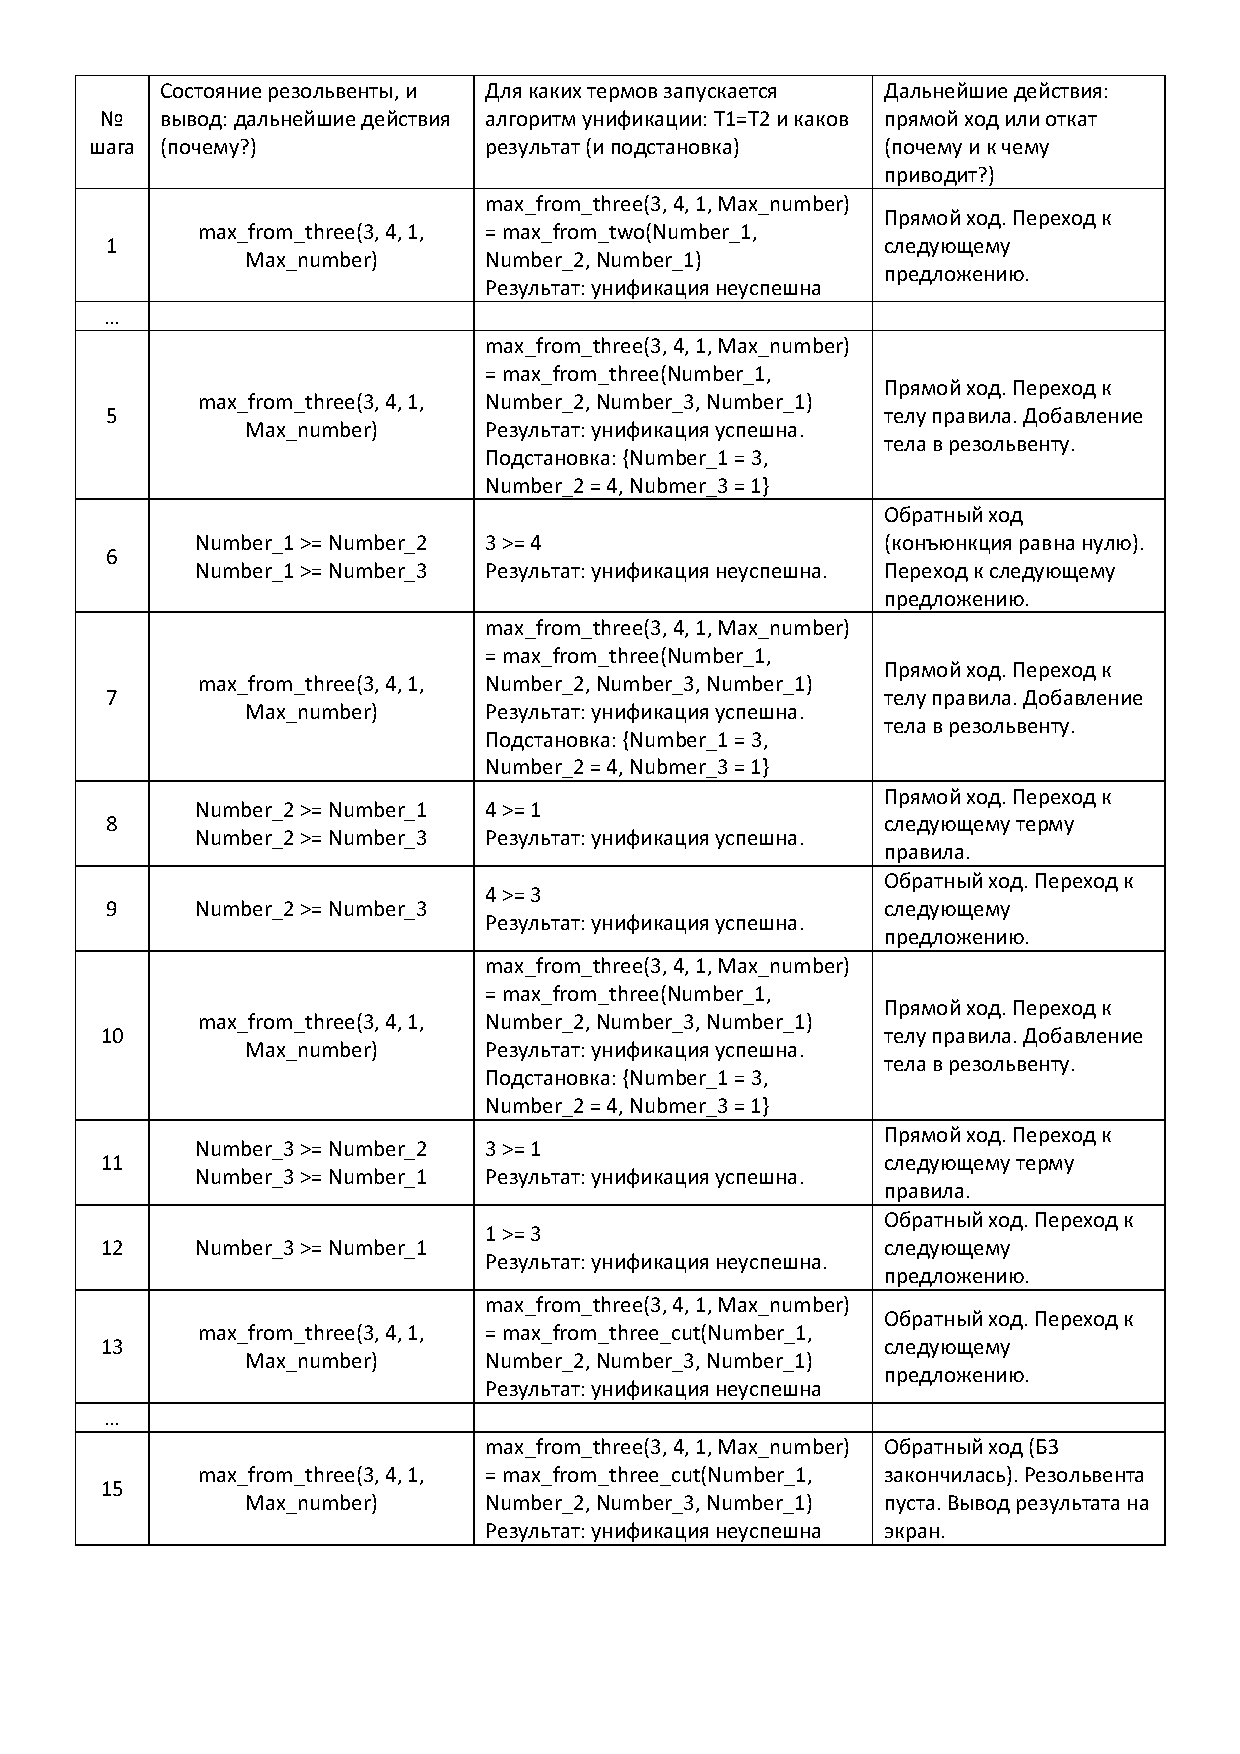
\includegraphics[scale=0.92]{images/table_5_1.pdf}
		\caption{Таблица порядка поиска ответов для задания 2 (без отсечения).}
		\label{image:table_1}
	}
\end{figure}
Ниже на рисунке \ref{image:table_2} приведена таблица порядка поиска ответа для задания 2 (с отсечением):
\begin{figure}[H]
	\centering{
		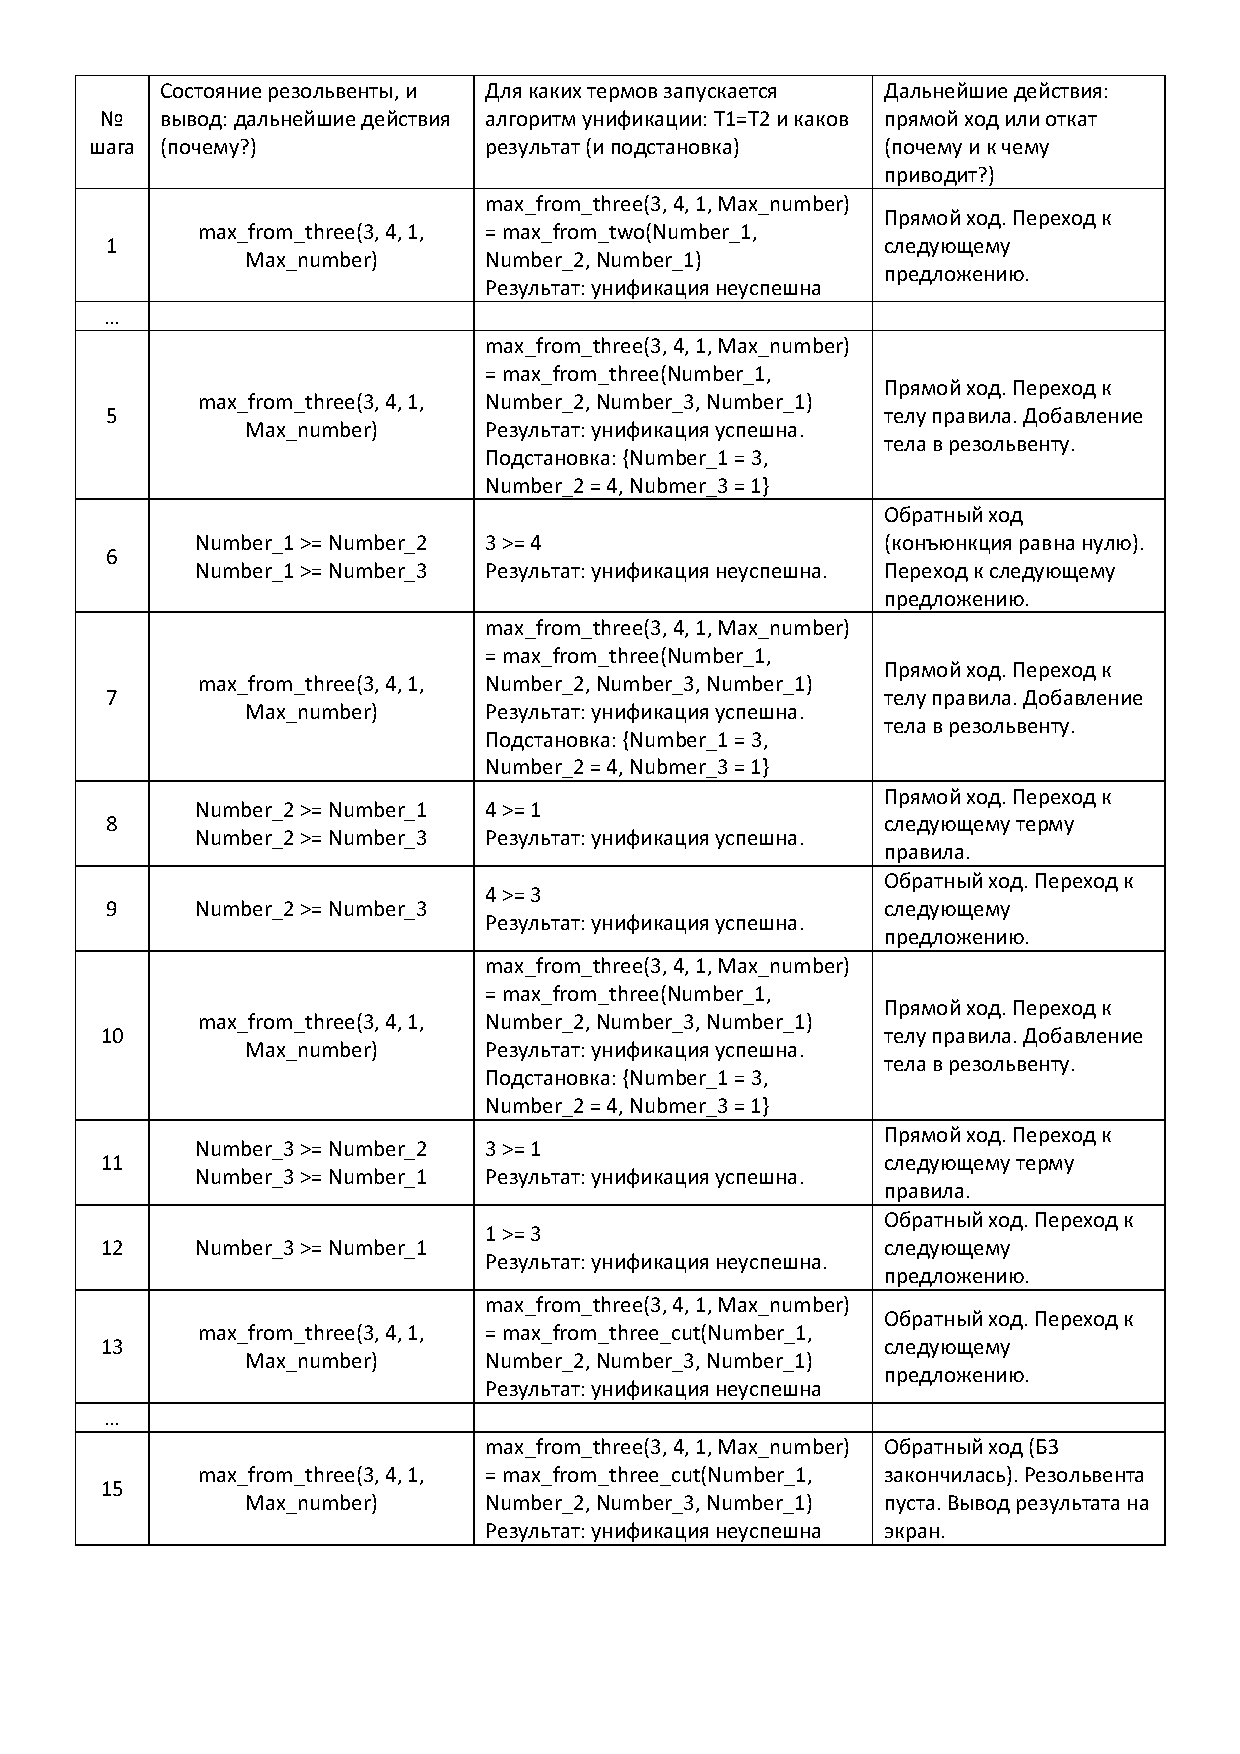
\includegraphics[scale=0.92]{images/table_5_1.pdf}
		\caption{Таблица порядка поиска ответов для задания 2 (с отсечением).}
		\label{image:table_2}
	}
\end{figure}